\documentclass[smaller,xcolor=dvipsnames]{beamer}
%\usepackage[orientation=portrait, size=a0, scale=1.4]{beamerposter}
\usecolortheme[named=RoyalBlue]{structure}
\usepackage[latin1]{inputenc}
\usepackage{MnSymbol,wasysym}
\usepackage[T1]{fontenc}
\usepackage{graphics}
\usepackage{movie15,amsmath}
\usepackage{graphicx}
\usepackage[all]{xy}
\usepackage{MnSymbol,wasysym}
\usepackage{tabularx,longtable,multirow,subfigure,caption}
%\usepackage[most]{tcolorbox}
%\usepackage{movie15}
%\usepackage{beamerthemesplit}
%\usetheme{Frankfurt}
%\usepackage[french]{babel}
%\usetheme {PaloAlto}
\usetheme{Warsaw}
%\usetheme{Madrid}
%\usetheme{Marburg}
%\DeclareGraphicsExtensions{eps,pdf,ps,jpg}
\newtheorem{question}{Question}
%\setbeamercolor{question}{bg=OliveGreen}
\newtheorem{questions}{Questions}
\newtheorem{proposition}{Proposition}
\newtheorem{remark}{Remark}
%\setbeamercolor{questions}{bg=OliveGreen}
\setbeamercolor{alerted text}{fg=RoyalPurple}
\newtheorem{idea}{Idea}
\setbeamercolor{idea}{bg=orange}
\makeatletter
\newcommand*{\compress}{\@minipagetrue}
\makeatother


\newcommand{\gln}{GL$_{n}(\mathbb{R})$}
\newcommand{\sln}{SL$_n(\mathbb{R})$}
\newcommand{\son}{SO$_{n}(\mathbb{R})$}

\title{Manifolds and homogeneous spaces \\(M2R2)}
\author{Xu Jiacheng, Zhang Dingxuan, Ameena Hassan, Jiang Shumin     \\ Supervised by: Dr. Marie-Amelie Lawn}
\institute{Imperial College London}
\date{16/06/2021}

\begin{document}

\begin{frame}{M2R Oral Presentation}
\titlepage    
\end{frame}

\begin{frame}{Outline}
 \tableofcontents
\end{frame}


\section{Brief definitions}
\subsection{Group actions on sets}
\begin{frame}{Group action on sets}
 \begin{block}{Deifinition}
An \textbf{action} of a group $G$ on a set $X$ is a map $\pi :G \times X \rightarrow X$, such that $\pi(g,x) = g \cdot x$ and satisfies the properties:\\
\pause
\begin{enumerate}
    \item $e_G \cdot x = x$, where $e_G$ is the identity element of $G$\\
    \pause
    \item For all $g_1,g_2 \in G$, $g_1 \cdot (g_2 \cdot x) = (g_1 \cdot g_2) \cdot x \hspace{20}$ 
\end{enumerate}
 \end{block}\\
\pause
Examples:\\
\pause
\begin{enumerate}
    \item The symmetric group $S(n)$ acts on the set $\{1,2,...,n\}$ by the various permutation maps;\\
    \pause
    \item The multiplicative group $R^{\ast}$ acts on the Euclidean space \rn\ by the scalar multiplication map.
\end{enumerate}
\end{frame}

\begin{frame}{Transitive actions}
\textbf{Having defining the group actions, we are interested in a particular type of them.}
\pause\\
\begin{block}{Definition}
A group action $G \times X \rightarrow X$ is called a \textbf{transitive} action if there exists $x\in X$ such that $X = G\cdot x = \{g\cdot x\ |\ g\in G\}$, where $G\cdot x$ is called the \textbf{G-orbit of x}.
\end{block}
\pause
\vspace{0.5cm}
Example:\\
\pause
We want to look at transitive actions acting on a n-sphere, but before that we need to know what a n-sphere is.\\
\pause
${S^{n}}\subset \mathbb{R}^{n+1}$ is defined as the set: $\{ x\in\mathbb{R}^{n+1}: \|x\| = 1 \}$, and can also be called the \textbf{n-sphere}.

\end{frame}

\begin{frame}{Transitive actions}
There are $9$ transitive actions on a $n-$sphere...\\
\pause
\vspace{0.5cm}
\begin{tabularx}{1\textwidth} { 
  | >{\centering\arraybackslash}X 
  | >{\centering\arraybackslash}X 
  | >{\centering\arraybackslash}X 
  | >{\centering\arraybackslash}X |}
 \hline
 Group & SO(n) & U(n), SU(n) & Sp(n)Sp(1), Sp(n)U(1), Sp(n) \\
 \hline
 Sphere  & S^{n-1}  & S^{2n-1} & S^{4n-1} \\
\hline
\end{tabularx}\\
\begin{center}
\begin{tabularx}{0.5\textwidth} { 
  | >{\centering\arraybackslash}X 
  | >{\centering\arraybackslash}X 
  | >{\centering\arraybackslash}X  |}
 \hline
 G_2 & Spin(7) & Spin(9) \\
 \hline
 S^6  & S^7  & S^{15} \\
\hline
\end{tabularx}
\end{center}
\end{frame}

\subsection{Homeomorphism}
\begin{frame}{Homeomorphism}
Homeomorphism \textcolor{red}{\textbf{(not homomorphism!)}} is an important concept to describe the mapping between two topological spaces.\\
\pause
\begin{block}{Definition}
A \textbf{homeomorphism} between two topological spaces $X,Y$ is a continuous bijection $f: X \rightarrow Y$ whose inverse is also continuous.\\
\pause
\vspace{0.5cm}
A \textbf{diffeomorphism} is a smooth homeomorphism whose inverse is also smooth.
\end{block}
\end{frame}
\subsection{Charts and atlases}
\begin{frame}{Charts and atlases}
\begin{block}{Definition}
A \textbf{chart} $(U,\varphi)$ for a topological space $X$ is a homeomorphism $\varphi$ from an open $U$ is a subset of $X$ to an open subset $\tilde{U}$ contained in $\mathbb{R}$, that is $\varphi : U \rightarrow \tilde{U}$.\\
\pause
\vspace{0.5cm}
An \textbf{atlas} for a topological space $X$ is the collection of charts for $X$ which covers $X$.
\end{block}
\end{frame}

\begin{frame}{Example}
\textbf{Consider the simple 2-sphere} $S^2$.\\
\pause
\begin{figure}[tb]
\centering
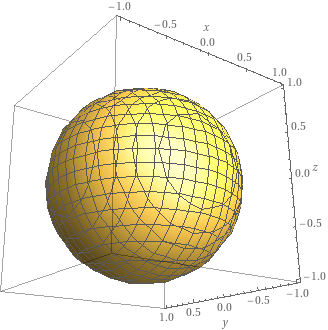
\includegraphics[width=40mm]{3d sphere.png} 
\caption{An atlas of the 2-sphere}
\end{figure}\\
\pause
$\varphi_{front}(x,y,z) = (x,z),\ \varphi_{left}(x,y,z) = (y,z), \ \varphi_{top}(x,y,z) = (x,y)...$
\end{frame}

\subsection{Paracompactness}
\begin{frame}{Paracompactness}
    \begin{block}{Definition}
    A topological space $X$ is \textbf{paracompact} if every open cover of $X$ has a locally finite open refinement.\\
    \pause
    \vspace{0.5cm}
    For a cover $C = \{U_\alpha : \alpha \in A \}$ of a topological space X, a \textbf{refinement} $D = \{V_\beta : \beta \in B \}$ of the cover $C$ is a subcover such that for all $V_\beta$ in $D$, exists $U_\alpha $ in $C \hspace{5}$ such that $ V_\beta \subseteq U_\alpha$.\\
    \pause
    \vspace{0.5cm}
    An open cover $C$ of $X$ is called \textbf{locally finite} if for all $x$ in $X$, exists $B(x)$ in $X$ where $B(x)$ is a neighbourhood of $x$ such that $B(x)$ intersects a finite number of subsets of $C$.
    \end{block}
\end{frame}

\begin{frame}{Paracompactness}
\begin{block}{Proposition}
Every compact space is paracompact.
\end{block}\\
\pause
\vspace{1cm}
\textcolor{red}{\textbf{However, the Euclidean space} $\mathbb{R}^n$ \textbf{is paracompact but not compact!}}

\end{frame}

\section{Manifolds}
\begin{frame}{Manifolds}
\textcolor{blue}{\textbf{What are manifolds?}}
\pause
\vspace{0.5cm}
\\
A manifold is a topological space that {\bf locally resembles} Euclidean space.
\pause
\begin{minipage}[t]{1\linewidth}
\vspace{1cm}
\centering
\fbox{\parbox{\textwidth}{
A topological space $X$ is {\bf Locally Euclidean of dimension $n$} if:\\
\\
For $p\in X$, there exists an open neighbourhood of $p$ that is homeomorphic to an open subset of $\mathbb{R}^{n}$
}}
\end{minipage}
\\
\vspace{1cm} \pause
\textcolor{red}{\textbf{Recall definition of charts. Every point in locally Euclidean space is contained in some charts.}}\\
\end{frame}

\subsection{Topological Manifolds}
\begin{frame}{Topological manifolds}
 \begin{block}{Definition}
A {\bf topological manifold} $M$ is a topological space if it is:\\
\pause
\begin{enumerate}
    \item {\bf Hausdorff}: For every $x$ and $y$ in $M$ with $x \neq y$, there are open sets $U$ and $V$ such that $x \in U$, $y \in V$, and $U \cap V=\emptyset$.
    \pause \\
    \item {\bf Second countable}: $M$ has a countable basis, which means there exists a countable collection $\mathbb{B}$ of open subsets of $M$ such that for any open subset $U$ of $M$ and point $p$ in $U$, there is an open set $B \in \mathbb{B}$ such that $p \in B \subset U$.
    \pause \\
    \item {\bf Locally Euclidean}: For every point $p\in M$, there exists a neighbourhood $N$ of $p$ such that $N$ is homeomorphic to an open subset of \rn.
    \end{enumerate}.
    \end{block}

\end{frame}

\begin{frame}{Examples}
The trivial $\mathbb{R}^{n}$ is a topological space since it satisfies the three properties in the definition.
\\
\pause \\
\begin{block}{Proposition}
Subspace of Hausdorff and second-countable space is also Hausdorff and second-countable.
\end{block}

\end{frame}

\begin{frame}{Examples}
\textcolor{blue}{Another example is the {\bf unit n-sphere} $S^{n}=\{x\in \mathbb{R}^{n+1}: |x| = 1\}$.} \\
\pause
Let $U_i=\{(x_1,…,x_{n+1})\in S^n:x_i>0\}$ and $V_i=\{(x_1,…,x_{n+1})\in S^n:x_i<0\}$
\begin{figure}
\centering
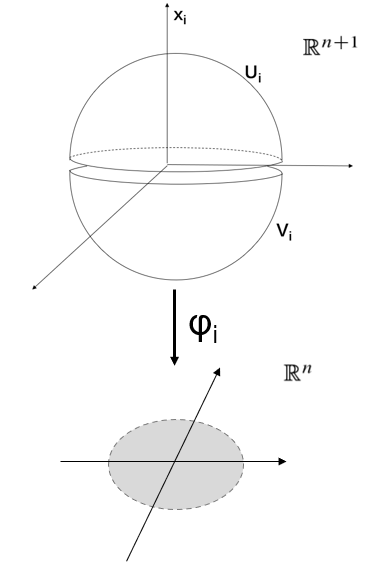
\includegraphics[width=33mm]{projection of charts of n-sphere.png} 
\caption{projection of charts of n-sphere}
\end{figure}
\end{frame}

\subsection{Smooth manifolds}
\begin{frame}{Transition map}
\begin{block}{Definition}
For two charts $(U,\varphi)$ and $(V,\psi)$ in a topological manifold, we say if U and V are not disjoint then the composition map $\varphi$$\circ$$\psi ^ {-1}:\psi(U\cap V)\rightarrow \varphi(U\cap V)$, or $\psi$$\circ$$\varphi ^ {-1}:\varphi(U\cap V)\mapsto \psi(U\cap V)$ defined on the intersection of U and V is a \textbf{transition map}. 
\end{block}
\end{frame}

\begin{frame}{Transition map}
    \begin{figure}[tb]
\centering
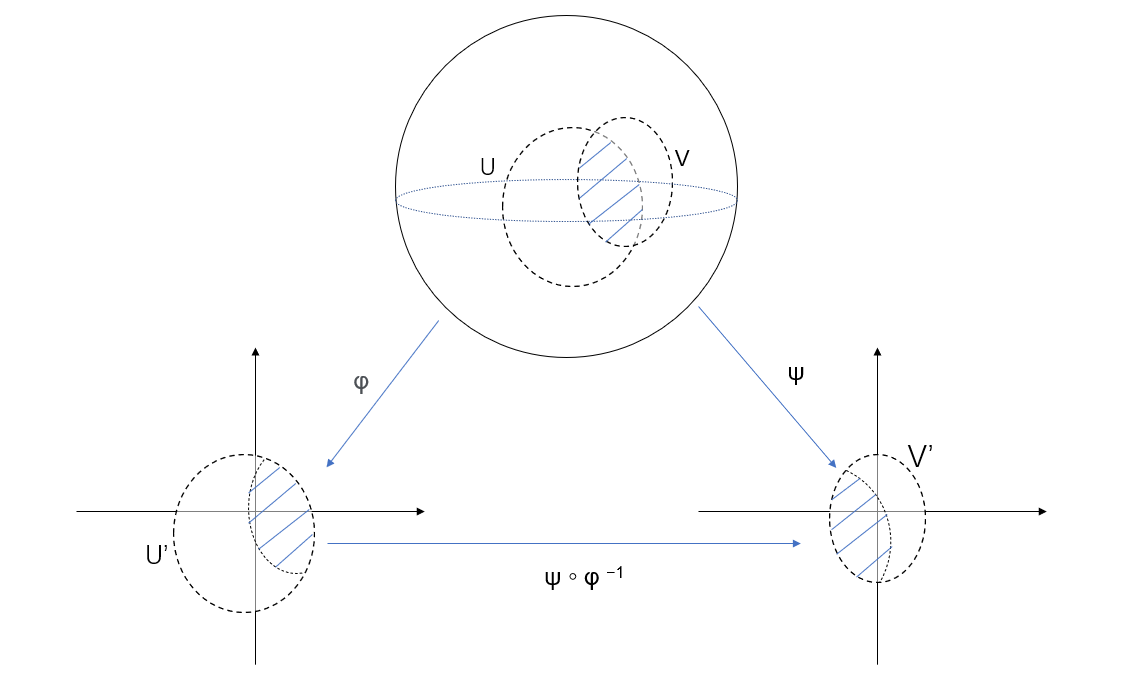
\includegraphics[width=90mm]{transition map.png} 
\caption{transition map}
\end{figure}
\end{frame}

\begin{frame}{Smooth Atlas}
    We say two charts $(U,\varphi)$ and $(V,\psi)$ are {\bf smoothly compatible} if either they are disjoint or their transition map is a diffeomorphism.\\
    \pause
    \begin{block}{Definition}
    An atlas is a {\bf smooth atlas} if every chart of it is smoothly compatible with each other.
    \end{block}

\end{frame}

\begin{frame}{Smooth manifolds}
    \begin{block}{Definition}
A {\bf smooth manifold} is a pair $(M,\mathbb{A})$ where $\mathbb{A}$ is a maximal(not contained in any larger smooth atlas) smooth atlas on a topological manifold $M$.
    \end{block}
    \vspace{1cm}
    \pause
Examples: $\mathbb{R}^n$, n-sphere,\gln,...
\end{frame}

\section{Lie Groups}
\subsection{Intuition}
\begin{frame}{Intuition}
\textcolor{blue}{\textbf{What are Lie groups?}}
\end{frame}

\begin{frame}{Lie Groups}
    \begin{block}{Definition}
    A Lie group is a group $G$ that is also a smooth manifold and the map $G \rightarrow G$, $(g,h)\mapsto gh^{-1}$, with $g,h\in G$ is smooth.
    \end{block}
    \pause\\
    Result from Analysis 2: the composition of smooth maps is itself a smooth map 
\end{frame}

\subsection{Examples}


\begin{frame}{Some results:}
We have a few results already
\begin{itemize}
    \item \gln is a smooth manifold
    \item The determinant map: $\det: GL_{n}(\mathbb{R}) \rightarrow \mathbb{R}$ is a smooth map
    \item Taking the inverse of a matrix is a smooth map
    \item Matrix multiplication is a smooth map
    \item The orthogonal group map $A \mapsto AA^{\top}$ is continuous. 
\end{itemize}
    
\end{frame}

\begin{frame}{}
    \begin{figure}
        \centering
        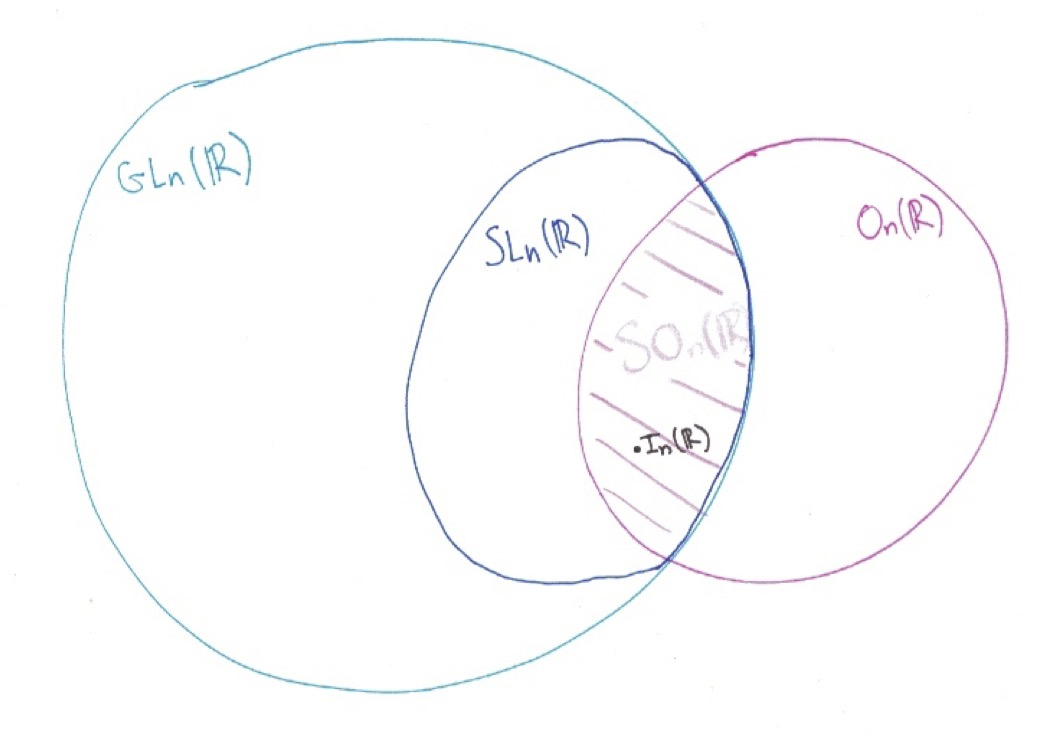
\includegraphics[height=7cm,width=11cm]{Lie_group_diagram.jpg}
        \caption{A visual representation of groups we claim are Lie groups}
        \label{fig:LieGroupFig}
    \end{figure}
\end{frame}

\begin{frame}{Some results:}
We have a few results already:
\begin{itemize}
    \item \gln is a smooth manifold
    \item The determinant map: $\det: GL_{n}(\mathbb{R}) \rightarrow \mathbb{R}$ is a smooth map
    \item Taking the inverse of a matrix is a smooth map
    \item Matrix multiplication is a smooth map
    \item The orthogonal group map $A \mapsto AA^{\top}$ is continuous. 
    \item The preimage of a continuous function on a closed set is also a closed set
\end{itemize}
\begin{block}{E. Cartan Closed subgroup Theorem}
Any closed subgroup $H$ of a Lie group $G$ is a Lie subgroup and hence a submanifold of $G$.
\end{block}
\end{frame}

\begin{frame}{Examples of Lie groups}
    \begin{block}{Example: \gln}
    \begin{itemize}
        \item Matrix multiplication, taking the inverse is smooth
        \item \gln is a smooth manifold
        \item \textbf{\gln is a Lie group}
    \end{itemize}
    \end{block}
    \pause
    \begin{block}{Example: \sln}
    \begin{enumerate}
        \item \sln is a subgroup of \gln
        \pause 
        \item \sln = $\det^{-1}\{1\}$ is a topologically closed subgroup because \pause preimage of a continuous function on a closed set is also closed
        \pause
        \item Apply E. Cartan's Closed subgroup theorem\pause
        \item \textbf{\sln is a Lie subgroup} and submanifold of \gln\pause 
        \item Matrix multiplication and taking inverse are smooth maps in \sln \implies \sln is also a smooth manifold
    \end{enumerate}
    \end{block}
\end{frame}

\begin{frame}{Examples of Lie groups}



\newcommand{\on}{$O_n(\mathbb{R})$}
\begin{block}{Definition: \on}
\on is the set of all matrices, that, when multiplied by their own inverse, give the identity matrix
\end{block}
\begin{block}{Definition: \son}
\son  is the set of all $n\times n$ invertible matrices with $\det = 1$ and the inverse of each matrix is itself.
\end{block}
\end{frame}

\begin{frame}{Examples of Lie groups}
    
\begin{block}{Example: \son}
\begin{enumerate}
    \item \son is a subgroup of \sln
    \item Taking the transverse is a continuous map on $O_n$.
    \item $O:SL_n(\mathbb{R}) \rightarrow SL_n(\mathbb{R}),\ O(A) = AA^{\top}$ also acts on \son (as determinant 1 is preserved), 
    \item $SO_n(\mathbb{R})$ = $O^{-1}(\{I_n\})$. As $\{I_n\}$ is closed in $SL_n(\mathbb{R})$, the preimage $SO_n(\mathbb{R})$ is also (topologically) closed
    \item Apply E. Cartan's Closed subgroup theorem
    \item \textbf{\son is a Lie subgroup} and submanifold of \sln
    \item Matrix multiplication and taking inverse are smooth maps in \son \implies \son is also a smooth manifold
\end{enumerate}
\end{block}
\end{frame}

\section{Homogeneous spaces}
\subsection{Isotropy group}
\subsection{Homogeneous space}
\subsection{Homogeneous space and principal bundles}
\begin{frame}{What is Isotropy group}
    The definition of isotropy group helps understand our main example of homogeneous space, and it's defined as follows:
\pause
    \begin{definition}
    An \textbf{isotropy group} $G_{x}$ is a subgroup of G, which for all $g$ in $G_{x},\ g\cdot x=x$.
    \end{definition}
\pause
    The main result here is the special linear group $SO(n)$ is the isotropy group of $SO(n+1)$.
\begin{figure}[tb]
\centering
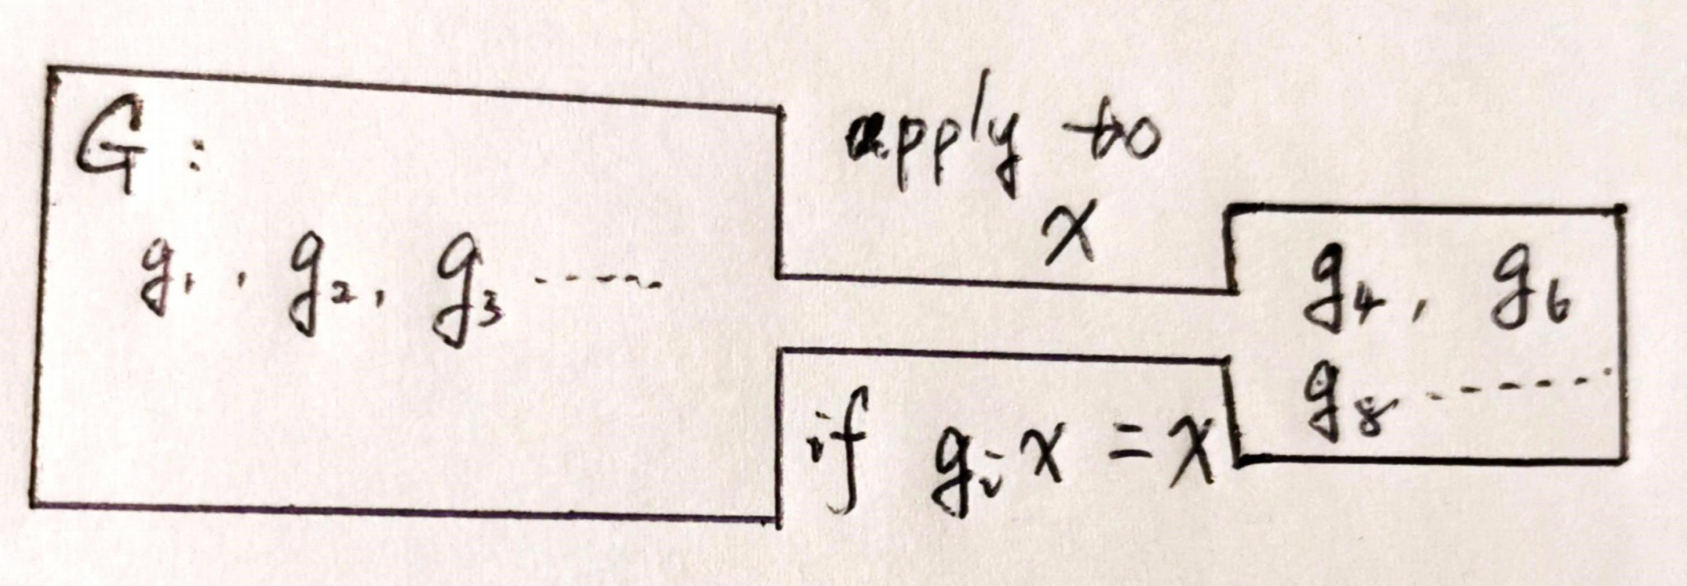
\includegraphics[width=90mm]{iso.png} 
\caption{Isotropy group}
\end{figure}
\end{frame}

\begin{frame}{Homogeneous space}
    \begin{definition}
    \textbf{Homogeneous space:} A homogeneous space for a group G can be a smooth manifold, or in general a topological space X on which G acts transitively.
    \end{definition}
\pause
    An example of homogeneous space would be $S^{n}$\\
\pause
    Proof is straight-forward using results from previous slides, but note that it's slightly different from the definition, the ingredients we need:\\
\pause
    1. Lie group action acts transitively on $G$.\\
    2. $S^{n}$ is a smooth manifold.
    
\end{frame}

\begin{frame}{Homogeneous space}
\begin{figure}[tb]
\centering
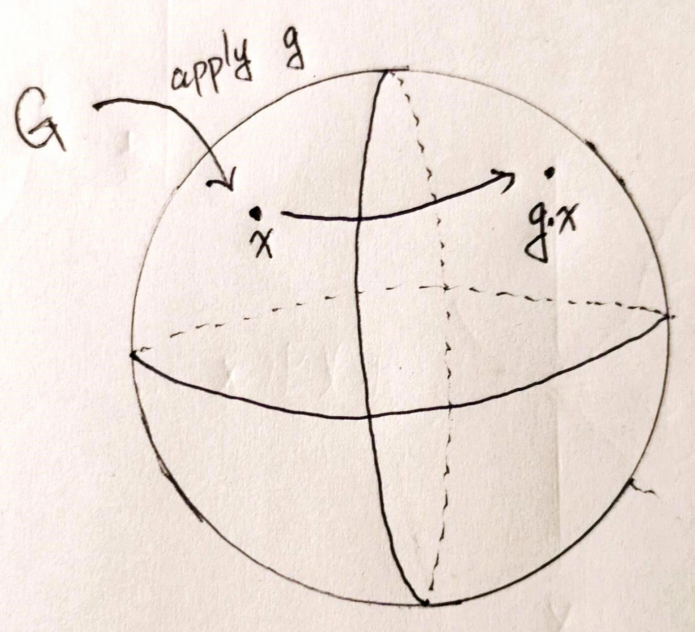
\includegraphics[width=60mm]{homo.png} 
\caption{Homogeneous space}
\end{figure}
\end{frame}

\begin{frame}{Homogeneous space and principal bundles}
First, definition of a fiber bundle:\\
    \begin{definition}
    For $E$ (total space), $B$ (base fiber), $F$ (fiber) topological spaces and a continuous map $\pi : E \rightarrow B$ form a \textbf{fiber bundle with fiber F} if:
    \begin{enumerate}
        \item B is a connected topological space.
        \item The natural projection map $\pi: E \rightarrow B$ is surjective.
        \item Each element in the base fiber has an open neighbourhood contained within the base fiber. That is for all $x \in B$, $\exists$ open neighbourhood $U_{x} \subset B$, there exists a homeomorphism $\varphi: \pi^{-1}(U_{x})\rightarrow U_{x}\times F$, that is a topological isomorphism.
    \end{enumerate}
    \end{definition}
\end{frame}

\begin{frame}{Homogeneous space and principal bundles}
    \begin{figure}[tb]
\centering
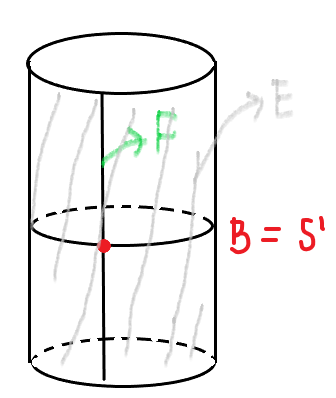
\includegraphics[width=40mm]{fiber bundle.png} 
\caption{Fiber bundle}
\end{figure}
\end{frame}

\newcommand{\iso}{\xrightarrow{
   \,\smash{\raisebox{-0.65ex}{\ensuremath{\scriptstyle\sim}}}\,}}
\begin{frame}{Homogeneous space and principal bundles}
    Principal bundle is the special case of fiber bundle, and here's the definition of principal bundles:
    \pause
    \begin{definition}
        \textbf{Principal bundles}: A principal G-bundle with a topological space G, is a fiber bundle $\pi:\ E\rightarrow B$, together with a continuous right action $\omega: E\times G \rightarrow E$, and that $\tilde{\pi}:= E\times G \xrightarrow{\mu} E \xrightarrow{\pi} B$ \newline{}and $E\times G \xrightarrow{\pi \times C} B \times \{e \} \iso B$ commutes with the map $C$, a map from everything to identity.
        And given a point $x\in B$, $G$ acts freely and transitively on the fiber $F_{x}$.
        

    \end{definition}
\end{frame}

\begin{frame}{Homogeneous space and principal bundles}
\begin{figure}[tb]
\centering
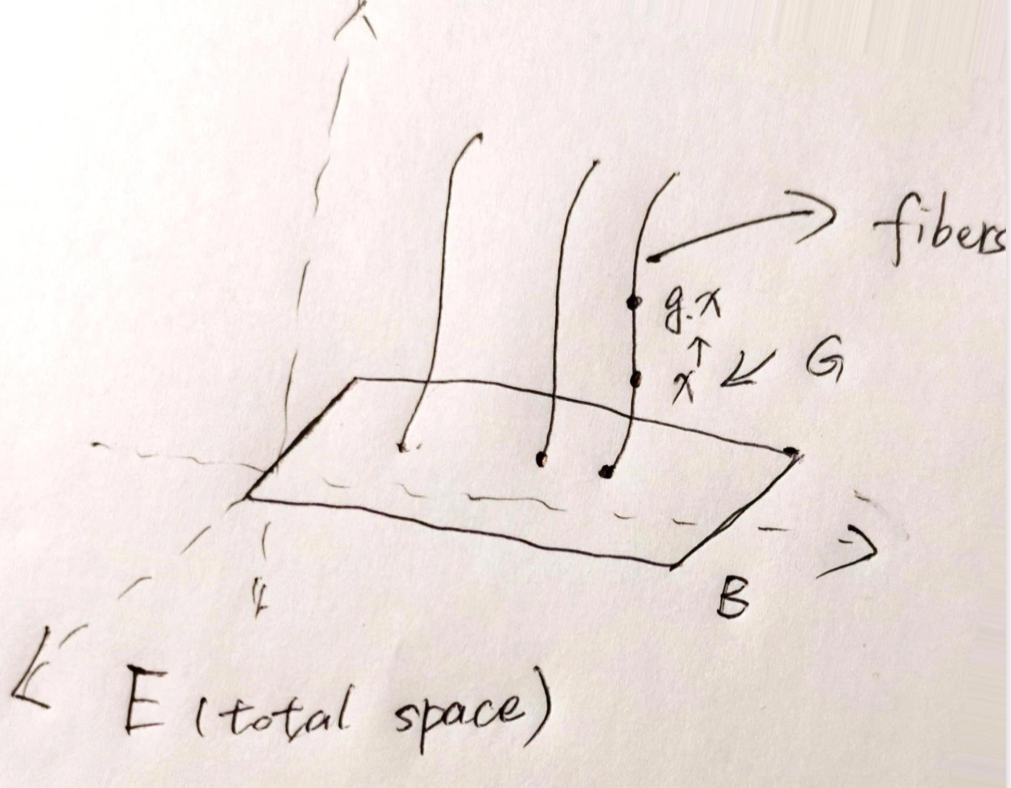
\includegraphics[width=90mm]{princ bun.png} 
\caption{Principal bundle}
\end{figure}
\end{frame}

\section{Applications}
\begin{frame}{Applications}
    \begin{itemize}
        \item Take isotropy group to be a fiber
        \item $G/G_{iso} \times G_{iso}$\\
        \pause
        \item Connections and parallel transport across manifolds\\
        \pause
        \item More applied areas, e.g. Mathematical gauge theory
    \end{itemize}
\end{frame}


\section{References}
\begin{frame}{References}
\begin{thebibliography}{999}
\bibitem{our paper}
Xu Jiacheng, Zhang Dingxuan, Ameena Hassan, Jiang Shumin. \textit{M2R2 Written Report 2020-21} Imperial College London [Accessed from 16th June 2021]
\bibitem{geom homog}
Andreas Cap. \textit{Geometry of homogeneous spaces}[Lecture] University of Vienna. Spring 2019
\end{thebibliography}
\end{frame}

\end{document}

